\subsection{Feuer- und Rauchsimulationen}

\subsubsection{Eigenschaften}
Chemische Reaktionen wie Feuer, oder der aus winzigen Partikeln bestehende Rauch,
lassen sich nur schwer physikalisch exakt simulieren. Es haben sich hierfür verschiedene Ansätze entwickelt, um ein
annähernd realistisches Rendering dieser Phänomene (mit volumetrischem Charakter) zu erschaffen. 
Es gibt hierbei beispielsweise die physikalisch basierten Ansätze. 
Diese beruhen auf aufwändig berechneten Fluidsimulationen und werden vorallem in der Gefahrensimulation verwendet.
Diese sind aufgrund ihrer Komplexität aber nur bedingt echtzeitfähig und werden meist zuvor berechnet. 
Der Fokus liegt dabei meist auf der realistischen Ausbreitung des Feuers und des Rauchs, um beispielsweise Fluchtwege 
zu testen oder Evakuierungsszenarien zu simulieren. Diese Anwendungsfälle müssen nicht in Echtzeit berechnet werden.
Daher ist diese Art der Simulation auch für Anwendungen, in denen es um die Interaktion mit dem Feuer geht, nicht 
effizient nutzbar. Ein Beispiel dafür ist der Einsatz in einem Simulator, der den Umgang mit dem Feuerlöscher
näher bringen soll. Diese basieren zumeist auf effizienteren Partikelsystemen, mit denen sich solche Phänomene 
durch eine Vielzahl an Parametern ebenfalls darstellen lassen. Dieser Ansatz ist dabei eher von artistischer Natur. 
Partikel lassen sich zwar genau steuern, beispielsweise durch Vektorfelder. Um ein realistisches Aussehen zu 
erzeugen gibt es aber vorallem in Videospielen andere Methoden, die sich durchgesetzt haben. 

Feuer, bzw. Flammen sind brennende, Licht und Wärme emittierende Gase, erzeugt durch eine chemische Reaktion. 
Feuer brennt für gewöhnlich mit Temperaturen zwischen 500°C und 1400°C, was einem Farbspektrum von dunkelrot bis hin zu weiß entspricht \parencite{Schmidt2011}.
Hierbei kommt es allerdings immer auch auf den Stoff an, der verbrannt wird.  
Durch die Verbrennung werden viele, winzige Rußpartikel in die Umgebung abgegeben. Durch ihre Leichtigkeit und den 
Auftrieb der Hitze verteilen sich diese in einer Wolke nach oben. Dies drückt sich in Form einer dunklen Wolke aus.
Obwohl beide Phänomene einhergehen, können diese Vorgänge als getrennte Partikelsysteme betrachtet werden.
Dennoch laufen oftmals beide Volumen ineinander über. Auch können sich – aufgrund von Turbulenzen – einzelne Flammen bei größerem Feuer lösen
und aufsteigen (vgl. \textbf{\autoref{fig:explosion}}).
Daher sollten die beiden Systeme für realistische Darstellungen von Bränden immer zusammen abgebildet werden.

\begin{figure}[h!]
	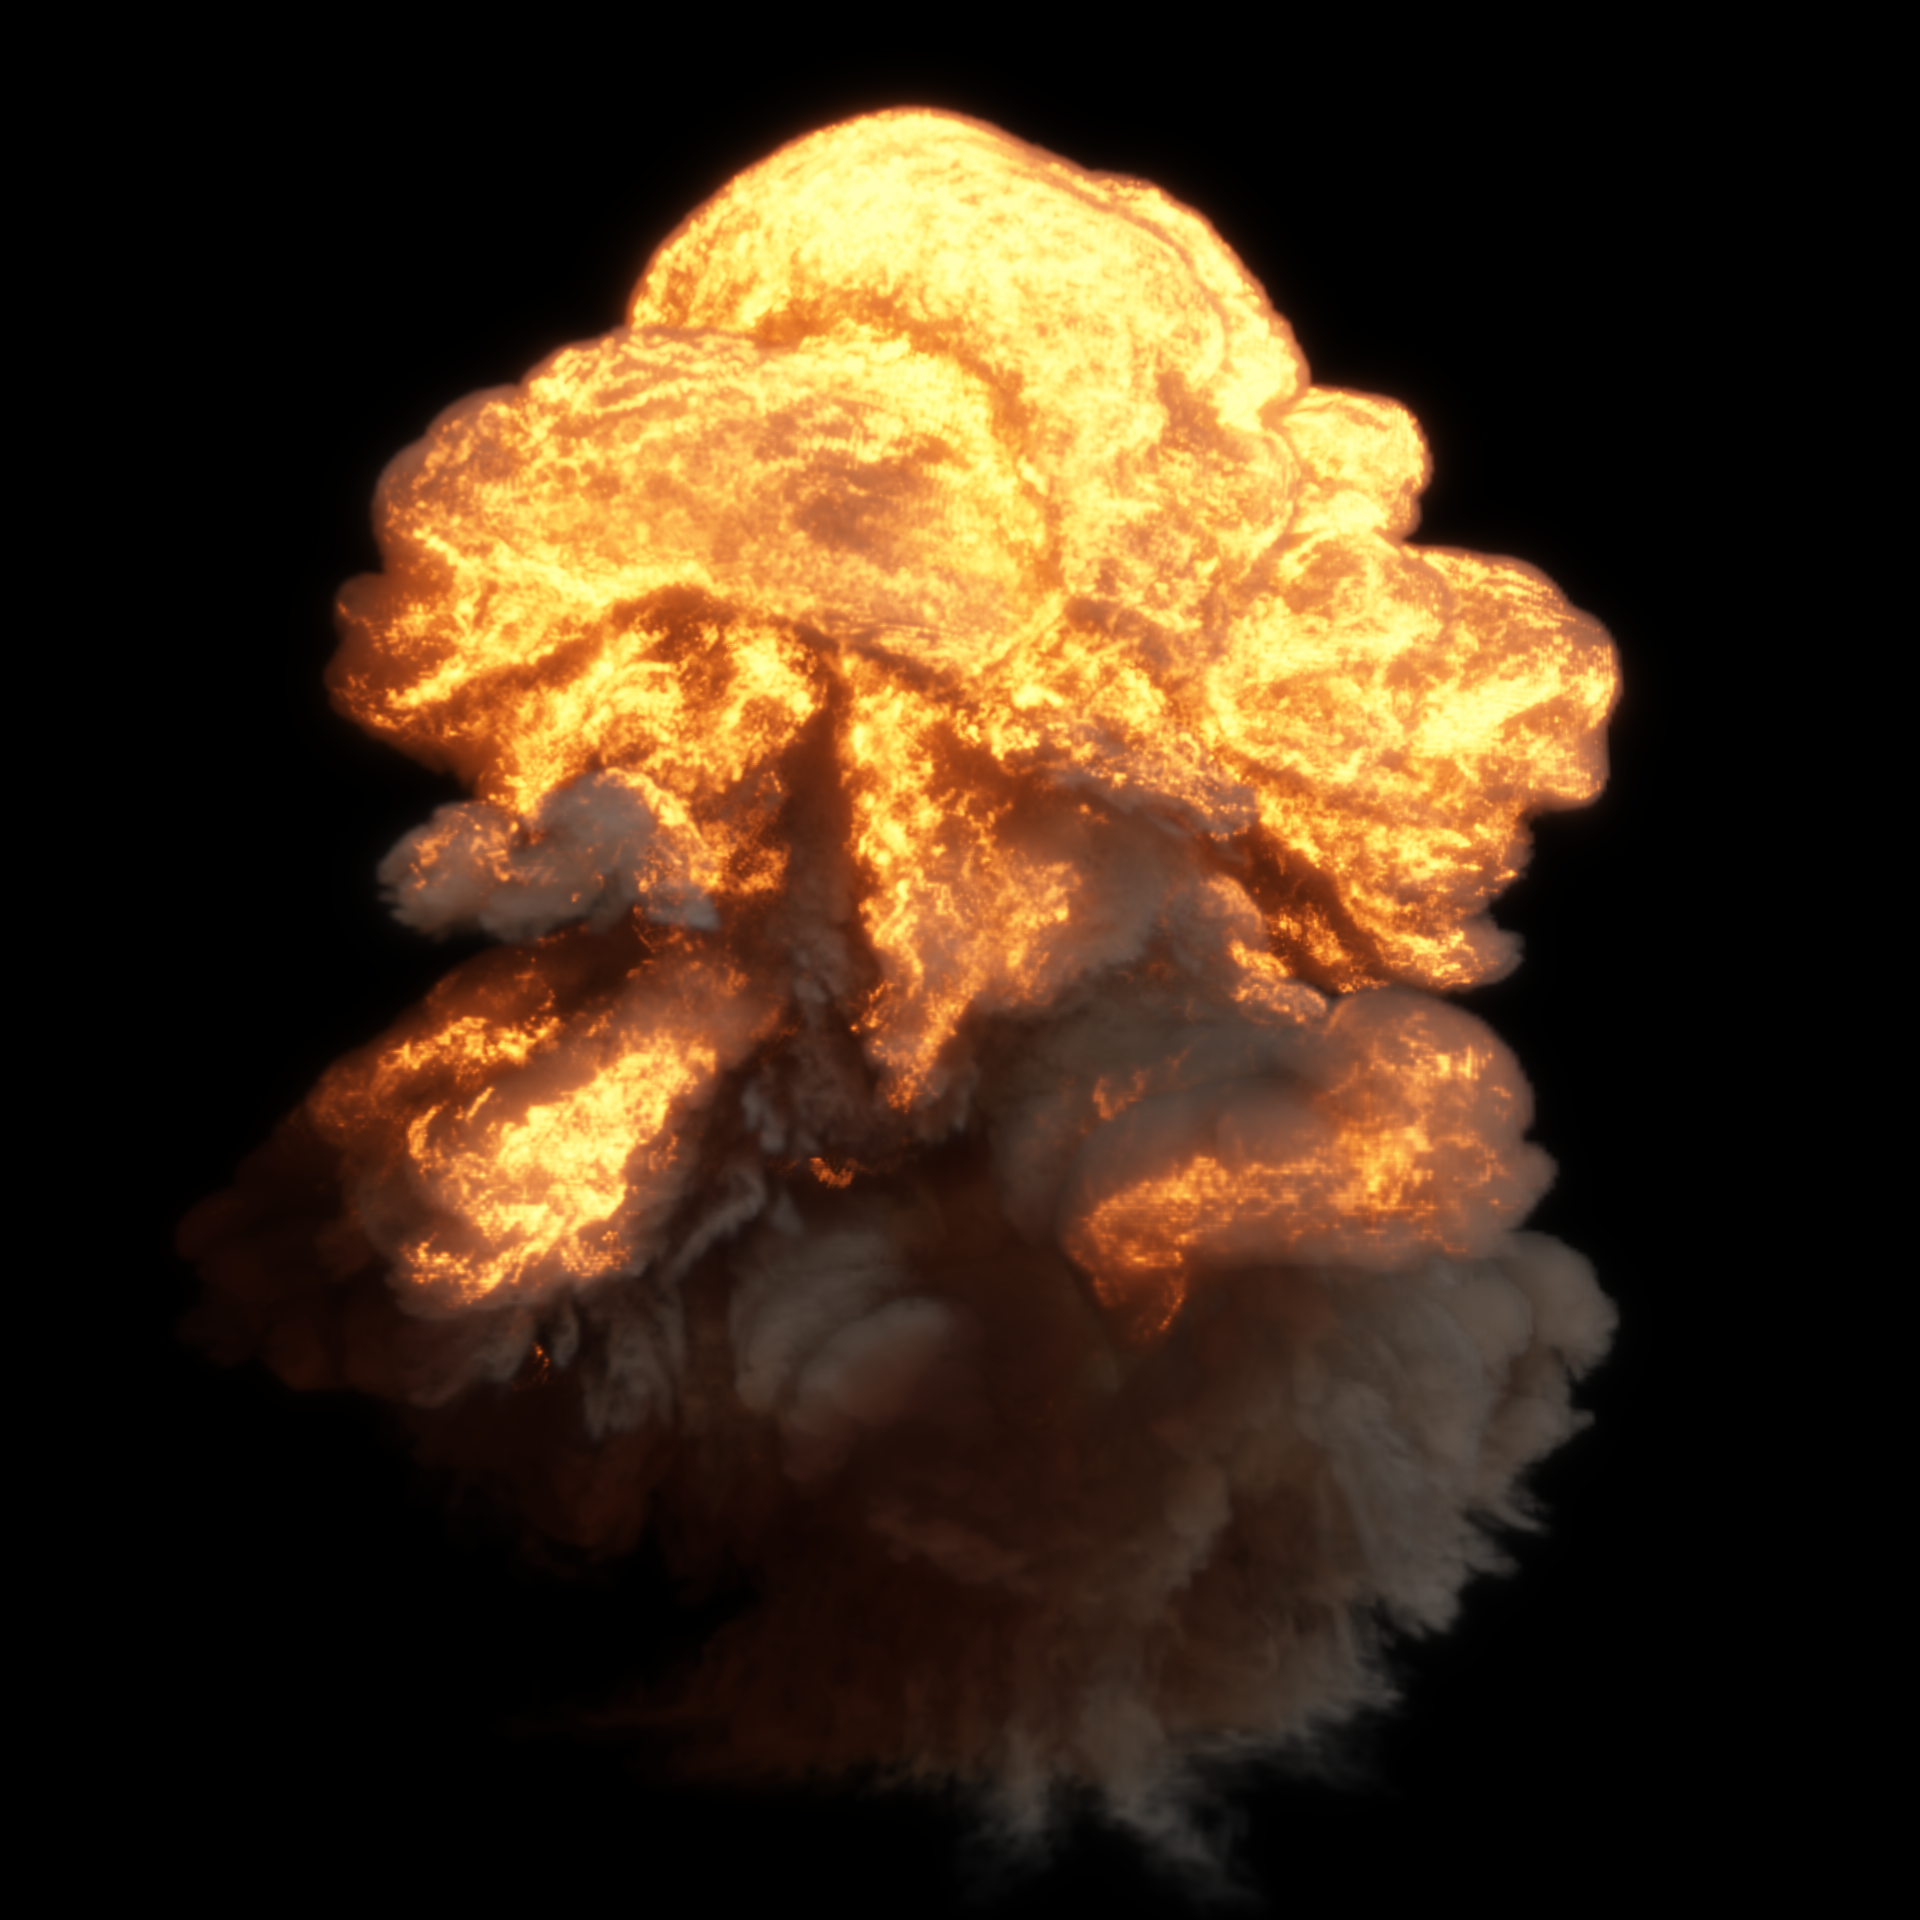
\includegraphics[width=0.49\textwidth]{Grafiken/Basics/Fire/explosion_0000.png}
	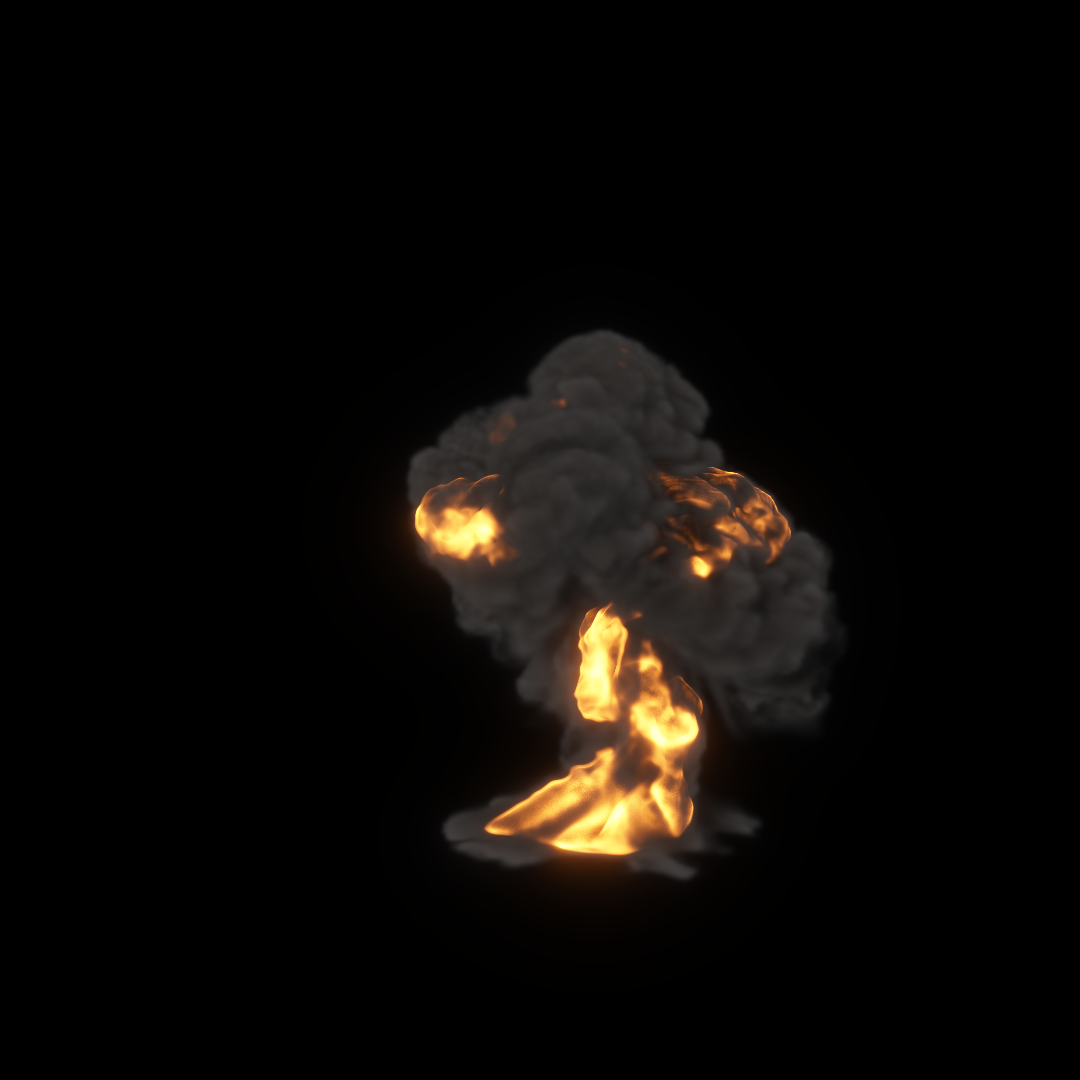
\includegraphics[width=0.49\textwidth]{Grafiken/Basics/Fire/explosion2_0000_0000.png}
	\centering
	\begin{footnotesize}
		\caption{Physikalisches Rendering von Feuer. Simuliert in EmberGen von JangaFX.  
			Links: Rendering einer Explosion. Rechts: Zu erkennen sind hier die einzelnen Flammen, die sich loslösen und nach oben steigen.}
		
		\label{fig:explosion}
	\end{footnotesize}
\end{figure}


\subsubsection{Partikelsysteme}
Partikelsysteme sind Methoden, mit denen sich solche Phänomene, die normalerweise schwer, beziehungsweise gar nicht, realistisch 
als Geometrie darzustellen sind, simulieren. Dazu gehören neben Feuer und Rauch auch Haare, Staub und andere visuelle Effekte.

Ein Partikelsystem besteht aus einem Emitter, der viele einzelne Partikel erzeugen kann. Diese werden mit einigen Eigenschaften ausgestattet. Darunter
bspw. die Lebensdauer, die Art des Partikels, die initiale Geschwindigkeit und die Richtung, in der die Partikel ausgestoßen werden oder etwa die Größe \parencite{Reeves1983}.
Alle diese Parameter lassen sich über die Zeit, bzw. die Lebensdauer der Partikel animieren. 
So können die Partikel ein- und ausgeblendet werden, sie können über die Zeit auch größer, heller oder langsamer werden. 
Um die Partikelsimulation für ein Feuer möglichst realistisch zu machen, können die Parameter auch randomisiert werden und manipuliert werden.
Partikel können auf physikalische Gegebenheiten, wie Collisionen oder Schwerkraft reagieren. Alle diese Optionen machen Partikelsysteme zu einem 
Werkzeug, um verschiedenste Objekte oder Effekte darzustellen, die sich durch Meshes nicht darstellen lassen könnten. 

Einzelne Partikel können durch verschiedenste Arten dargestellt werden. Zu diesen Arten gehören Punkte, Linien, Sprites oder Meshes.
Für Feuer und Rauch hat sich der Einsatz von Sprites, oder auch Billboards, durchgesetzt. Billbords sind simple, meistens quadratische, texturierte Polygone,
die sich zum Betrachter ausrichten, sodass dieser die Sprites jederzeit von vorne sieht. Durch die ständige Korrektur der Ausrichtung fällt
nicht auf, dass die gesehenen Partikel komplett flach sind. Aus diesem Grund lassen sich volumetrische Effekte mit Billboard-basierten Partikeln, 
auf einen zweidimensionalen Bildschirm projiziert, gut vortäuschen.  Die Texturen lassen sich zudem animieren, was die Illusion noch mehr verstärkt.  
Dafür werden keine Rechenressourcen bezüglich des Renderings von echten Volumen nötig, der Effekt ist jedoch vergleichbar.
